\chapter{Diferenciální počet}

\begin{prolog}
:- ensure_loaded("../equations/formula").

make_test_real_numbers([-2, -1, 0, 1, 1.5, 2]).
make_test_real_nonzero_numbers([-2, -1, 1, 1.5, 2]).
make_test_natural_numbers([1, 2, 3, 4, 5]).
make_test_real_functions(FX, [FX, FX^2, FX + 1, (FX + 1) * FX^5]).

make_test_functions_with_limit(
	X,
	[
		(X + 1) * X / X,
		(X + 1) * (X - 2) * (X^2 - 4) / (X^2 - 4)
	]
).

make_test_nonzero_functions_with_limit(
	X,
	[
		(X^2 + 1) * X / X,
		(-(X+2)^2 - 3) * (X^2 - 4) / (X^2 - 4)
	]
).

make_test_positive_functions_with_limit(
	X,
	[
		(X^2 + 1) * X / X,
		((X+2)^2 + 3) * (X^2 - 4) / (X^2 - 4)
	]
).

make_test_continuous_functions(
	X,
	[
		X,
		2 * X,
		X / 2,
		X^2,
		X^3,
		sin(X),
		cos(X)
	]
).

make_test_continuous_functions_nonzero_derivative(
	X,
	[
		sin(X) + 2*X,
		cos(X) - 3*X
	]
).

make_test_continuous_2d_functions(
	X, Y,
	[
		X^2 * Y,
		sin(X) * cos(Y),
		cos(X) * sin(2 * Y),
		sin(X) + cos(Y)
	]
).

make_test_2d_functions_with_limit(
	X, Y,
	[
		X * ((X - 1)^2 + (Y + 1)^2) / ((X - 1)^2 + (Y + 1)^2),
		(X + Y^2 + 1) * (X^2 + Y^2) / (X^2 + Y^2)
	]
).

make_test_points([0, 2, -2, 1]).
\end{prolog}

Diferenciální počet se zabývá chováním funkcí při malých změnách jejich parametrů. Budeme tedy zkoumat, jak se funkce chovají v~okolí nějakého bodu.

\section{Limita funkce}

V~metrickém prostoru \((M, d)\) pro \(\delta > 0\) definujme \(\delta\)-okolí prvku \(P \in M\) jako množinu bodů, jejichž vzdálenost od prvku \(P\) je menší než \(\delta\):

\begin{equation}
\forall \delta > 0, P \in M: U_{\delta}(P) = \{X \in M: d(X, P) < \delta\}
\end{equation}

Zaveďme také označení pro výlučné \(\delta\)-okolí prvku \(P\), tedy okolí bez vlastního bodu:

\begin{equation}
\overset{\circ}{U}_{\delta}(P) = U_{\delta}(P) \setminus P
\end{equation}

Pokud v~dalším textu neuvedeme jinak, tak za metrický prostor budeme považovat Euklidovský prostor. Budeme tedy používat metriku \eqref{eq:euklidovsky_prostor_metrika} i~v~případě, že ji bude nutné zavést uměle. V~Euklidovském prostoru představuje  \(\delta\)-okolí obecně hyperkouli okolo zvoleného bodu. V~jednorozměrném prostoru se jedná o~interval \(|x - x_0| < \delta\), ve dvojrozměrném prostoru o~kruh \((x - x_0)^2 + (y - y_0)^2 < \delta^2\) a~ve třírozměrném prostoru o~kouli \((x - x_0)^2 + (y - y_0)^2 + (z - z_0)^2 < \delta^2\).

Limitou funkce \(y = \lim_{P \to P_0} \mathrm{f}(P)\) rozumíme to, k~jaké funkční hodnotě se funkce blíží, pokud se její argumenty \(P\) blíží k~bodu \(P_0\). Přesná definice je následující. To, že funkce \(\mathrm{f}(P)\) má v~bodě \(P_0\) limitu \(y\) znamená, že pro každé kladné \(\varepsilon\) lze nalézt kladné \(\delta\) takové, že funkce má ve výlučném \(\delta\)-okolí bodu \(P_0\) hodnoty ležící v~\(\varepsilon\)-okolí bodu \(y\):

\begin{equation}
\forall \varepsilon > 0 \; \exists \delta > 0 \; \forall P \in \overset{\circ}{U}_{\delta}(P_0) \; \mathrm{f}(P) \in U_{\varepsilon}(y)
\end{equation}

Limitu tedy můžeme dokázat tak, že nalezneme funkci \(\delta(\varepsilon)\) splňující výše uvedené požadavky.

Na funkční hodnotě v~daném bodě nezáleží. Funkce nemusí být ani v~daném bodě definovaná. Metrický prostor funkčních argumentů a~funkčních hodnot je obecně různý.

Funkce nemusí mít v~daném bodě limitu, pokud ji však má, tak je tato limita jednoznačně určená. Dokažme to. Předpokládejme, že \(\lim_{x \to x_0} = a\) a~\(\lim_{x \to x_0} = b\), přičemž \(a \neq b\). Pak \(\mathrm{d}(a, b) > 0\) je vzdálenost mezi funkčními hodnotami \(a\) a~\(b\). Potom při volbě \(\varepsilon = \left| \frac{\mathrm{d}(a, b)}{2} \right|\) budou \(\varepsilon\)-okolí bodů disjunktní. Díky podmínce \eqref{eq:pseudometricky_prostor_definice_3} pro metrický prostor totiž nemůže existovat funkční hodnota \(c\), aby \(\mathrm{d}(a, c) < \varepsilon\) a~\(\mathrm{d}(b, c) < \varepsilon\). Tím je dokázáno, že v~jednom bodě nemohou existovat 2 různé limity.

Na obrázku \ref{img:limita_funkce} jsou zobrazeny 3 funkce, které všechny mají v~bodě \(x = 1\) limitu 1. První funkce je spojitá, druhá funkce nemá funkční hodnotu v~daném bodě definovanou, třetí funkce má v~daném bodě jinou funkční hodnotu než limitu. Naopak na obrázku~\ref{img:neexistence_limity} jsou zobrazeny 3 funkce, které nemají v~bodě \(x = 1\) limitu. První funkce má v~tomto bodě "skok". Druhá funkce není částečně v~okolí bodu definovaná. Třetí funkce v~tomto bodě roste nede všechny meze. V~tomto případě říkáme, že funkce má nevlestní limitu a~zapisujeme to \(\lim_{x \to 1} \mathrm{f}(x) = \infty\). Přesnou definicí nevlestní limity se nebudeme zabývat.
 
\begin{figure}
\begin{center}
\begin{tikzpicture}

// Spojita funkce
\tikzmath{ \x = 0; \y = 0; }

\draw[->] (\x - 0.5, \y) -- (\x + 2.5, \y);
\draw (\x + 2.5, 0) node[anchor=north]{x};

\draw[->] (\x, \y - 0.5) -- (\x, \y + 2.5);
\draw (\x, \y + 2.5) node[anchor=east]{y};

\draw (\x, \y) -- (\x + 2, \y + 2);

\draw[dashed] (\x + 1, \y) -- (\x + 1, \y + 1) -- (\x, \y + 1);
\draw (\x + 1, \y) node[anchor=north]{1};
\draw (\x, \y + 1) node[anchor=east]{1};

// Funkce s vyloucenym bodem
\tikzmath{ \x = 3.5; \y = 0; \r = 0.05;}

\draw[->] (\x - 0.5, \y) -- (\x + 2.5, \y);
\draw (\x + 2.5, 0) node[anchor=north]{x};

\draw[->] (\x, \y - 0.5) -- (\x, \y + 2.5);
\draw (\x, \y + 2.5) node[anchor=east]{y};

\draw (\x, \y) -- (\x + 1 - \r * 0.70711, \y + 1 - \r * 0.70711);
\draw (\x + 1 + \r * 0.70711, \y + 1 + \r * 0.70711) -- (\x + 2, \y + 2);

\draw (\x + 1, \y + 1) circle[radius=\r];

\draw[dashed] (\x + 1, \y) -- (\x + 1, \y + 1) -- (\x, \y + 1);
\draw (\x + 1, \y) node[anchor=north]{1};
\draw (\x, \y + 1) node[anchor=east]{1};

// Funkce s jinym bodem
\tikzmath{ \x = 7; \y = 0; \r = 0.05;}

\draw[->] (\x - 0.5, \y) -- (\x + 2.5, \y);
\draw (\x + 2.5, 0) node[anchor=north]{x};

\draw[->] (\x, \y - 0.5) -- (\x, \y + 2.5);
\draw (\x, \y + 2.5) node[anchor=east]{y};

\draw (\x, \y) -- (\x + 1 - \r * 0.70711, \y + 1 - \r * 0.70711);
\draw (\x + 1 + \r * 0.70711, \y + 1 + \r * 0.70711) -- (\x + 2, \y + 2);

\draw (\x + 1, \y + 1) circle[radius=\r];
\draw[fill=black] (\x + 1, \y + 2) circle[,radius=\r];

\draw[dashed] (\x + 1, \y) -- (\x + 1, \y + 1) -- (\x, \y + 1);
\draw (\x + 1, \y) node[anchor=north]{1};
\draw (\x, \y + 1) node[anchor=east]{1};

\end{tikzpicture}
\caption{Limita funkce}
\end{center}
\label{img:limita_funkce}
\end{figure}

\begin{figure}
\begin{center}
\begin{tikzpicture}

// Funkce se skokem
\tikzmath{ \x = 0; \y = 0; \r = 0.05;}

\draw[->] (\x - 0.5, \y) -- (\x + 2.5, \y);
\draw (\x + 2.5, 0) node[anchor=north]{x};

\draw[->] (\x, \y - 0.5) -- (\x, \y + 2.5);
\draw (\x, \y + 2.5) node[anchor=east]{y};

\draw (\x, \y + 1) -- (\x + 1, \y + 2);
\draw (\x + 1 + \r * 0.70711, \y + 1 + \r * 0.70711) -- (\x + 2, \y + 2);

\draw (\x + 1, \y + 1) circle[radius=\r];
\draw[fill=black] (\x + 1, \y + 2) circle[,radius=\r];

\draw[dashed] (\x + 1, \y) -- (\x + 1, \y + 2);
\draw (\x + 1, \y) node[anchor=north]{1};

// Funkce bez okoli
\tikzmath{ \x = 3.5; \y = 0; \r = 0.05;}

\draw[->] (\x - 0.5, \y) -- (\x + 2.5, \y);
\draw (\x + 2.5, 0) node[anchor=north]{x};

\draw[->] (\x, \y - 0.5) -- (\x, \y + 2.5);
\draw (\x, \y + 2.5) node[anchor=east]{y};

\draw (\x + 1, \y + 1) -- (\x + 2, \y + 2);

\draw[fill=black] (\x + 1, \y + 1) circle[,radius=\r];

\draw[dashed] (\x + 1, \y) -- (\x + 1, \y + 1);
\draw (\x + 1, \y) node[anchor=north]{1};

// Nevlastni limita
\tikzmath{ \x = 7; \y = 0; \r = 0.05;}

\draw[->] (\x - 0.5, \y) -- (\x + 2.5, \y);
\draw (\x + 2.5, 0) node[anchor=north]{x};

\draw[->] (\x, \y - 0.5) -- (\x, \y + 2.5);
\draw (\x, \y + 2.5) node[anchor=east]{y};

\draw[dashed] (\x + 1, \y) -- (\x + 1, \y + 2);
\draw (\x + 1, \y) node[anchor=north]{1};

\draw[domain=-0.5:0.7, smooth, variable = \t] plot ({\x + \t}, {\y + 1 / ((\t - 1) * (\t - 1)) / 5});
\draw[domain=1.3:2.3, smooth, variable = \t] plot ({\x + \t}, {\y + 1 / ((\t - 1) * (\t - 1)) / 5});

\end{tikzpicture}
\caption{Neexistence limity}
\end{center}
\label{img:neexistence_limity}
\end{figure}

\subsection{Spojitost funkce}
\label{sec:spojitost_funkce}

Funkci nazveme spojitou v~daném bodě pokud je limita v~tomto bodě rovna funkční hodnotě. Tedy pokud v~daném bodě funkce limitů má, má v~něm i~funkční hodnotu a~limita je funkční hodnotě rovna. Tedy pokud

\begin{equation}
\lim_{P \to P_0} \mathrm{f}(P) = \mathrm{f}(P_0)
\end{equation}

Není-li funkce v daném bodě definovaná, ale je možné ji upravit tak, že se v~okolí bodu nezmění a~po úpravě bude spojitá, pak můžeme její limitu vypočítat jako hodnotu této upravené funkce. Příklad:

\begin{prolog}
?-	print_validated_formula(
		"lim_continuity_example",
		equal([
			lim(X, "x", real, 0, (2 * X) / X),
			lim(X, "x", real, 0, 2),
			2
		])
	).
\end{prolog}
\eeq{lim_continuity_example}

\subsection{Příklad}

Dokažme

\begin{prolog}
?-	print_validated_formula(
		"lim_proof_example_1",
		equal([
			lim([X, Y], ["x", "y"], [real, real], [0, 2], (X^2 + X * Y) / X),
			2
		])
	).
\end{prolog}
\eeq{lim_proof_example_1}

\begin{prolog}
?-	make_test_real_numbers(Numbers),
	make_test_real_nonzero_numbers(NonzeroNumbers),
	print_validated_multiformula(
		[
			variable(DX, "\\mathrm{d}x", NonzeroNumbers),
			variable(DY, "\\mathrm{d}y", Numbers),
			substitution(X, "x", 0 + DX),
			substitution(Y, "y", 2 + DY),
			substitution(DELTA1, "\\Delta", abs(DX + DY)),
			substitution(DELTA2, "\\delta", max(set_of([abs(DX), abs(DY)]))),
			substitution(EPSILON, "\\varepsilon", 2 * DELTA2)
		],
		[
			formula(
				"lim_proof_example_2",
				equal([
					DELTA1,
					abs((X^2 + X * Y) / X - 2),
					abs(X + Y - 2),
					abs(DX + (2 + DY) - 2),
					abs(DX + DY)
				])
			),
			formula(
				"lim_proof_example_3",
				less_or_equal(
					DELTA1,
					2 * DELTA2
				)
			),
			formula(
				"lim_proof_example_3",
				equal(DELTA2, EPSILON / 2)
			),
			formula(
				"lim_proof_example_4",
				impl(
					less_than(sqrt(DX^2 + DY^2), DELTA2),
					less_than(DELTA1, EPSILON)
				)
			)
		]
	).
\end{prolog}

Nejdříve vyjádřeme vzdálenost funkce od předpokládané limity 2:
\eeq{lim_proof_example_2}

Vidíme, že pokud zvolíme
\eeq{lim_proof_example_3}

pak bude platit
\eeq{lim_proof_example_4}

a~hodnota limity je tak dokázána.

\subsection{Limita složené funkce}

Pro limitu složených funkcí platí následující vztah. Přitom předpokládáme, že hodnota funkce g (bod \(Q_0\)) leží ve stejném metrickém prostoru jako argument funkce f (bod \(Q\)), tedy že se v obou případech používá stejná metrika.

\begin{prolog}
?-	make_test_functions_with_limit(FP, FunctionsF),
	make_test_functions_with_limit(GP, FunctionsG),
	make_test_points(Points),
	print_validated_formula(
		"limita_slozene_funkce",
		declare(
			[
				variable(P0, "P_0", Points),
				function(F, "f", FunctionsF),
				function(G, "g", FunctionsG),
				substitution(Q0, "Q_0", lim(P, "P", real, P0, apply(G, [GP], [P]))),
				substitution(Y, "y", lim(Q, "Q", real, Q0, apply(F, [FP], [Q])))
			],
			impl(
				and(
					equal(lim(P, "P", real, P0, apply(G, [GP], [P])), Q0),
					equal(lim(Q, "Q", real, Q0, apply(F, [FP], [Q])), Y)
				),
				equal(lim(P, "P", real, P0, apply(F, [FP], [apply(G, [GP], [P])])), Y)
			)
		)
	).
\end{prolog}
\eeq{limita_slozene_funkce}

Pokud je funkce \(f\) spojitá, tak její limitu můžeme nahradit její funkční hodnotou a~vztah se zjednodušší:

\begin{prolog}
?-	make_test_continuous_functions(FP, FunctionsF),
	make_test_functions_with_limit(GP, FunctionsG),
	make_test_points(Points),
	print_validated_formula(
		"limita_spojite_slozene_funkce",
		declare(
			[
				variable(P0, "P_0", Points),
				function(F, "f", FunctionsF),
				function(G, "g", FunctionsG)
			],
			equal(
				lim(P, "P", real, P0, apply(F, [FP], [apply(G, [GP], [P])])),
				apply(F, [FP], [lim(P, "P", real, P0, apply(G, [GP], [P]))])
			)
		)
	).
\end{prolog}
\eeq{limita_spojite_slozene_funkce}

Obě dvě věty je třeba chápat jako implikace. Neexistence limit jednotlivých funkcí ještě neznemaná, že neexistuje limita složené funkce.

Přistupme k důkazu. Z~definice limit funkcí \(\mathrm{f}\) a~\(\mathrm{g}\) víme:

\begin{equation}
\begin{split}
\forall Q \in \overset{\circ}{U}_{\delta_f(\varepsilon_f)}(Q_0) \; \mathrm{f}(Q) \in U_{\varepsilon_f}(y) \\
\forall P \in \overset{\circ}{U}_{\delta_g(\varepsilon_g)}(P_0) \; \mathrm{g}(P) \in U_{\varepsilon_g}(Q_0)
\end{split}
\end{equation}

Uvědomíme-li si, že z~\(\varepsilon_g \leq \delta_f(\varepsilon_f)\) plyne

\begin{equation}
\overset{\circ}{U}_{\varepsilon_g}(Q_0) \subset \overset{\circ}{U}_{\delta_f(\varepsilon_f)}(Q_0)
\end{equation}

a~my můžeme první rovnici specializovat pokud zvolíme \(\varepsilon_g = \delta_f(\varepsilon_f)\):

\begin{equation}
\begin{split}
\forall Q \in \overset{\circ}{U}_{\delta_f(\varepsilon_f)}(Q_0) \; \mathrm{f}(Q) \in U_{\varepsilon_f}(y) \\
\forall Q \; Q \in \overset{\circ}{U}_{\delta_f(\varepsilon_f)}(Q_0) \impl \mathrm{f}(Q) \in U_{\varepsilon_f}(y)
\end{split}
\end{equation}

Rovnici jsme zapsali ve tvaru implikace, protože \(\forall A \in S \; p(A)\) je jen zjednodušený zápis pro \(\forall A \; A \in S \Rightarrow p(A)\). 

Dále pak můžeme dosadit \(Q = \mathrm{g}(P)\):

\begin{equation}
\forall P \; \mathrm{g}(P) \in \overset{\circ}{U}_{\delta_f(\varepsilon_f)}(Q_0) \impl \; \mathrm{f}(\mathrm{g}(P)) \in U_{\varepsilon_f}(y)
\end{equation}

Ve druhé rovnici také zavedeme substituci \(\varepsilon_g = \delta_f(\varepsilon_f)\):

\begin{equation}
\begin{split}
\forall P \in \overset{\circ}{U}_{\delta_g(\delta_f(\varepsilon_f))}(P_0) \; \mathrm{g}(P) \in U_{\delta_f(\varepsilon_f)}(Q_0) \\
\forall P \; P \in \overset{\circ}{U}_{\delta_g(\delta_f(\varepsilon_f))}(P_0) \impl \mathrm{g}(P) \in U_{\delta_f(\varepsilon_f)}(Q_0)
\end{split}
\end{equation}

Obě rovnice jsou ve tvaru 2 implikací a~je možné využít transitivitu implikací. Získáme tak rovnici:

\begin{equation}
\begin{split}
\forall P \; P \in \overset{\circ}{U}_{\delta_g(\delta_f(\varepsilon_f))}(P_0) \impl \mathrm{f}(\mathrm{g}(P)) \in U_{\varepsilon_f}(y) \\
\forall P \in \overset{\circ}{U}_{\delta_g(\delta_f(\varepsilon_f))}(P_0) \; \mathrm{f}(\mathrm{g}(P)) \in U_{\varepsilon_f}(y)
\end{split}
\end{equation}

Tím je dokázán vztah pro limitu složené funkce.

\subsection{Zůžení limity}

Mějme funkci dvou proměnných \(\mathrm{g}(a, b)\). Pak existují-li limity na levé straně následujících rovností, pak rovnosti platí:

\begin{prolog}
?-	make_test_2d_functions_with_limit(GA, GB, Functions),
	make_test_real_numbers(Numbers),
	print_validated_formula(
		"zuzeni_limity_fixace",
		declare(
			[
				variable(A0, "a_0", Numbers),
				variable(B0, "b_0", Numbers),
				function(G, "g", Functions)
			],
			equal([
				lim(A, "a", real, A0, lim(B, "b", real, B0, apply(G, [GA, GB], [A, B]))),
				lim([A, B], ["a", "b"], [real, real], [A0, B0], apply(G, [GA, GB], [A, B])),
				lim(A, "a", real, A0, apply(G, [GA, GB], [A, B0])),
				lim(B, "b", real, B0, apply(G, [GA, GB], [A0, B]))
			])
		)
	).
\end{prolog}
\eeq{zuzeni_limity_fixace}

\begin{prolog}
?-	make_test_2d_functions_with_limit(GA, GB, Functions),
	make_test_real_numbers(Numbers),
	print_validated_formula(
		"zuzeni_limity_stejne_promenne",
		declare(
			[
				variable(X0, "x_0", Numbers),
				function(G, "g", Functions)
			],
			equal([
				lim(A, "a", real, X0, lim(B, "b", real, X0, apply(G, [GA, GB], [A, B]))),
				lim([A, B], ["a", "b"], [real, real], [X0, X0], apply(G, [GA, GB], [A, B])),
				lim(X, "x", real, X0, apply(G, [GA, GB], [X, X]))
			])
		)
	).
\end{prolog}
\eeq{zuzeni_limity_stejne_promenne}

Důkaz je zřejmý, okolí bodů u~limit vpravo je podmnožinou okolí bodů u~limit vlevo.

\subsection{Základní limity}

Níže jsou uvedeny základní limity. Předpokládáme při tom, že limity podvýrazů existují. Vztahy jsou odvozeny ze vztahu~\eqref{eq:limita_spojite_slozene_funkce}.

\begin{prolog}
?-	make_test_functions_with_limit(FX, FunctionsF),
	make_test_functions_with_limit(GX, FunctionsG),
	make_test_real_numbers(Numbers),
	print_validated_formula(
		"lim_sum",
		declare(
			[
				variable(P0, "P_0", Numbers),
				function(F, "f", FunctionsF),
				function(G, "g", FunctionsG),
				plus_minus(PM)
			],
			equal(
				lim(P, "P", real, P0, plus_minus(apply(F, [FX], [P]), apply(G, [GX], [P]), PM)),
				plus_minus(lim(P, "P", real, P0, apply(F, [FX], [P])), lim(P, "P", real, P0, apply(G, [GX], [P])), PM)
			)
		)
	).
\end{prolog}
\eeq{lim_sum}

\begin{prolog}
?-	make_test_functions_with_limit(FX, FunctionsF),
	make_test_functions_with_limit(GX, FunctionsG),
	make_test_real_numbers(Numbers),
	print_validated_formula(
		"lim_multiply",
		declare(
			[
				variable(P0, "P_0", Numbers),
				function(F, "f", FunctionsF),
				function(G, "g", FunctionsG)
			],
			equal(
				lim(P, "P", real, P0, apply(F, [FX], [P]) * apply(G, [GX], [P])),
				lim(P, "P", real, P0, apply(F, [FX], [P])) * lim(P, "P", real, P0, apply(G, [GX], [P]))
			)
		)
	).
\end{prolog}
\eeq{lim_multiply}

\begin{prolog}
?-	make_test_functions_with_limit(FX, Functions),
	make_test_nonzero_functions_with_limit(GX, NonzeroFunctions),
	make_test_real_numbers(Numbers),
	print_validated_formula(
		"lim_divide",
		declare(
			[
				variable(P0, "P_0", Numbers),
				function(F, "f", Functions),
				function(G, "g", NonzeroFunctions)
			],
			impl(
				not_equal(lim(P, "P", real, P0, apply(G, [GX], [P])), 0),
				equal(
					lim(P, "P", real, P0, apply(F, [FX], [P]) / apply(G, [GX], [P])),
					lim(P, "P", real, P0, apply(F, [FX], [P])) / lim(P, "P", real, P0, apply(G, [GX], [P]))
				)
			)
		)
	).
\end{prolog}
\eeq{lim_divide}

\begin{prolog}
?-	make_test_functions_with_limit(FX, Functions),
	make_test_real_numbers(Numbers),
	print_validated_formula(
		"lim_power_by_natural",
		declare(
			[
				variable(P0, "P_0", Numbers),
				function(F, "f", Functions)
			],
			forall_in(N, "n", natural_numbers, Numbers,
				equal(
					lim(P, "P", real, P0, apply(F, [FX], [P])^N),
					lim(P, "P", real, P0, apply(F, [FX], [P]))^N
				)
			)
		)
	).
\end{prolog}
\eeq{lim_power_by_natural}

\begin{prolog}
?-	make_test_positive_functions_with_limit(FX, PositiveFunctions),
	make_test_functions_with_limit(GX, Functions),
	make_test_real_numbers(Numbers),
	print_validated_formula(
		"lim_power_by_real",
		declare(
			[
				variable(P0, "P_0", Numbers),
				function(F, "f", PositiveFunctions),
				function(G, "g", Functions)
			],
			impl(
				greater_than(lim(P, "P", real, P0, apply(F, [FX], [P])), 0),
				equal(
					lim(P, "P", real(1e-10), P0, apply(F, [FX], [P])^apply(G, [GX], [P])),
					lim(P, "P", real, P0, apply(F, [FX], [P]))^lim(P, "P", real, P0, apply(G, [GX], [P]))
				)
			)
		)
	).
\end{prolog}
\eeq{lim_power_by_real}

\section{Derivace}

Derivací funkce rozumíme poměr změny funkční hodnoty vůči změne jejího parametru:

\begin{prolog}
?-	make_test_continuous_functions(FX, Functions),
	make_test_real_numbers(Numbers),
	print_validated_formula(
		"definice_derivace",
		declare(
			[
				function(F, "f", Functions),
				variable(X, "x", Numbers),
				substitution(Z, "z", apply(F, [FX], [X]))
			],
			proof([],
				[
					equal(Z, apply(F, [FX], [X])),
					equal(derivative(X, Z), lim(DX, "\\mathrm{d}x", real, 0, (apply(F, [FX], [X + DX]) - apply(F, [FX], [X])) / DX))
				]
			)
		)
	).
\end{prolog}
\eeq{definice_derivace}

V~literatuře se často derivace funkce jedné proměnné označuje \(\frac{\mathrm{d}z}{\mathrm{d}x}\), my se ale budeme držet výše uvedeného označení. 

Máme-li funkci více parametrů, pak ostatní parametry považujeme za konstantní. Takovou derivaci nazýváme parciální. Samozřejmě je možné vypočítat parciální derivace vůči všem parametrům:

\begin{prolog}
?-	make_test_continuous_2d_functions(FX, FY, Functions),
	make_test_real_numbers(Numbers),
	print_validated_formula(
		"definice_parcialni_derivace",
		declare(
			[
				function(F, "f", Functions),
				variable(X, "x", Numbers),
				variable(Y, "y", Numbers),
				substitution(Z, "z", apply(F, [FX, FY], [X, Y]))
			],
			proof([],
				[
					equal(Z, apply(F, [FX, FY], [X, Y])),
					equal(derivative(X, Z), lim(DX, "\\mathrm{d}x", real, 0, (apply(F, [FX, FY], [X + DX, Y]) - apply(F, [FX, FY], [X, Y])) / DX)),
					equal(derivative(Y, Z), lim(DY, "\\mathrm{d}y", real, 0, (apply(F, [FX, FY], [X, Y + DY]) - apply(F, [FX, FY], [X, Y])) / DY))
				]
			)
		)
	).
\end{prolog}
\eeq{definice_parcialni_derivace}

Je nutné mít na paměti, že \(\frac{\partial z}{\partial x}\) není podíl nebo zlomek, jedná se o symbol pro derivaci. Později sice uvidíme, že například derivace složené funkce vypadá jako krácení zlomků, ale ve skutečnosti je to opět jen symbolika zápisu.

\begin{figure}
\begin{center}
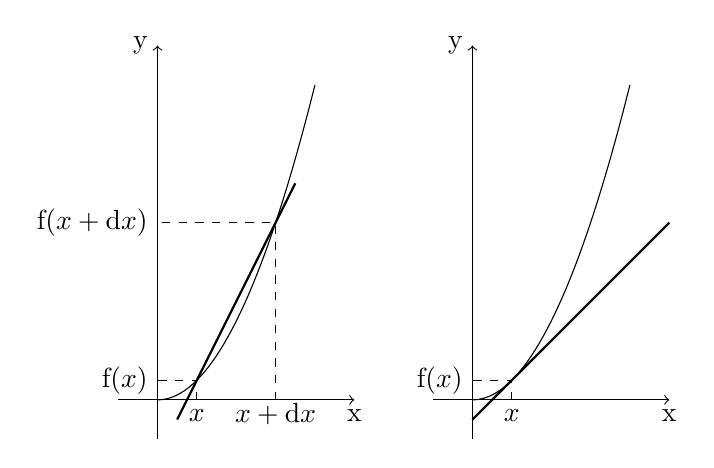
\begin{tikzpicture}
// Secna
\draw[->] (-0.5, 0) -- (2.5, 0);
\draw (2.5, 0) node[anchor=north]{x};

\draw[->] (0, -0.5) -- (0, 4.5);
\draw (0, 4.5) node[anchor=east]{y};

\draw[domain=0:2, smooth, variable = \x] plot ({\x}, {\x * \x});

\draw[thick] (0.25, -0.25) -- (1.75, 2.75); 

\draw[dashed] (0.5, 0) -- (0.5, 0.25) -- (0, 0.25);
\draw[dashed] (1.5, 0) -- (1.5, 2.25) -- (0, 2.25);

\draw (0.5, 0) node[anchor=north]{\(x\)};
\draw (1.5, 0.08) node[anchor=north]{\(x + \mathrm{d}x\)};

\draw (0, 0.25) node[anchor=east]{\(\mathrm{f}(x)\)};
\draw (0, 2.25) node[anchor=east]{\(\mathrm{f}(x + \mathrm{d}x)\)};

// Tecna
\draw[->] (3.5, 0) -- (6.5, 0);
\draw (6.5, 0) node[anchor=north]{x};

\draw[->] (4, -0.5) -- (4, 4.5);
\draw (4, 4.5) node[anchor=east]{y};

\draw[domain=0:2, smooth, variable = \x] plot ({\x + 4}, {\x * \x});

\draw[thick] (4.0, -0.25) -- (6.5, 2.25); 

\draw[dashed] (4.5, 0) -- (4.5, 0.25) -- (4, 0.25);

\draw (4.5, 0) node[anchor=north]{\(x\)};
\draw (4, 0.25) node[anchor=east]{\(\mathrm{f}(x)\)};

\end{tikzpicture}
\caption{Derivace funkce}
\end{center}
\label{img:derivace}
\end{figure}

Na obrázku \ref{img:derivace} je vidět grafický význam derivace. Přímka procházející body \([x, \mathrm{f}(x)]\) a~\([x + \mathrm{d}x, \mathrm{f}(x + \mathrm{d}x)]\) tvoří sečnu funkce \(\mathrm{f}\). Pokud \(\mathrm{d}x \to 0\), pak se sečna bude blížit tečně. Derivace proto představuje směrnici tečny v~daném bodě.

\subsection{Derivace složené funkce jedné proměnné}

Mějme složenou funkci

\begin{equation}
y = \mathrm{f}(\mathrm{g}(x))
\end{equation}

a~chtějme vypočítat její derivaci. Derivaci můžeme vypočítat podle definice~\eqref{eq:definice_derivace}:

\begin{prolog}
?-	make_test_continuous_functions(FX, FunctionsF),
	make_test_continuous_functions_nonzero_derivative(GX, FunctionsG),
	make_test_real_numbers(Numbers),
	print_validated_formula(
		"derivace_slozene_funkce_vypocet",
		declare(
			[
				function(F, "f", FunctionsF),
				function(G, "g", FunctionsG),
				variable(X, "x", Numbers),
				substitution(Y, "y", apply(F, [FX], [apply(G, [GX], [X])])),
				substitution(GV, "g", FX)   % Pojmenovany parametr funkce F kvuli derivaci
			],
			equal([
				derivative(X, Y),
				lim(DX, "\\mathrm{d}x", real, 0,
					(apply(F, [FX], [apply(G, [GX], [X + DX])]) - apply(F, [FX], [apply(G, [GX], [X])])) / DX
				),
				linebreak,
				lim(DX, "\\mathrm{d}x", real, 0, 
					((apply(F, [FX], [apply(G, [GX], [X + DX])]) - apply(F, [FX], [apply(G, [GX], [X])])) / DX) *
					(
						(apply(G, [GX], [X + DX]) - apply(G, [GX], [X])) / 
						(apply(G, [GX], [X + DX]) - apply(G, [GX], [X]))
					)
				),
				linebreak,
				lim(DX, "\\mathrm{d}x", real, 0, 
					((apply(F, [FX], [apply(G, [GX], [X + DX])]) - apply(F, [FX], [apply(G, [GX], [X])])) / (apply(G, [GX], [X + DX]) - apply(G, [GX], [X]))
				) *
					(
						(apply(G, [GX], [X + DX]) - apply(G, [GX], [X])) / 
						DX
					)
				),
				linebreak,
				lim(DX, "\\mathrm{d}x", real, 0, 
					((apply(F, [FX], [apply(G, [GX], [X + DX])]) - apply(F, [FX], [apply(G, [GX], [X])])) / (apply(G, [GX], [X + DX]) - apply(G, [GX], [X])))
				) *
				lim(DX, "\\mathrm{d}x", real, 0,
					(apply(G, [GX], [X + DX]) - apply(G, [GX], [X])) / 
					DX
				),
				linebreak,
				lim(DX, "\\mathrm{d}x", real, 0, 
					((apply(F, [FX], [apply(G, [GX], [X]) + apply(G, [GX], [X + DX]) - apply(G, [GX], [X])]) - apply(F, [FX], [apply(G, [GX], [X])])) / (apply(G, [GX], [X + DX]) - apply(G, [GX], [X])))
				) *
				lim(DX, "\\mathrm{d}x", real, 0,
					(apply(G, [GX], [X + DX]) - apply(G, [GX], [X])) / 
					DX
				),
				linebreak,
				lim(DG, "\\mathrm{d}g", real, 0, 
					(apply(F, [FX], [apply(G, [GX], [X]) + DG]) - apply(F, [FX], [apply(G, [GX], [X])])) / DG
				) *
				lim(DX, "\\mathrm{d}x", real, 0,
					(apply(G, [GX], [X + DX]) - apply(G, [GX], [X])) / 
					DX
				),
				linebreak,
				apply(derivative(GV, F), [FX], [apply(G, [GX], [X])]) * derivative(X, apply(G, [GX], [X]))
			])
		)
	).
\end{prolog}
\eeq{derivace_slozene_funkce_vypocet}

V~důkazu předpokládáme, že funkce \(g\) není v~okolí uvažovaného bodu konstantní a~proto \(g(x + \mathrm{d}x) \neq g(x)\). Pokud by funkce  \(g\) byla konstantní, pak by i~složená funkce \(f(g(x))\) byla konstantní a~uvedený vztah by také platil, protože jak funkce \(g\), tak složená funkce by měly nulové derivace. Několikrát jsme využili vztah pro limitu složené funkce~\eqref{eq:limita_slozene_funkce}.

Zapišme odvozený vztah ještě jednou, protože se jedná o~velmi důležitý vztah:

\begin{fact}
\begin{prolog}
?-	make_test_continuous_functions(FX, FunctionsF),
	make_test_continuous_functions(GX, FunctionsG),
	make_test_real_numbers(Numbers),
	print_validated_formula(
		"derivace_slozene_funkce",
		declare(
			[
				function(F, "f", FunctionsF),
				function(G, "g", FunctionsG),
				variable(X, "x", Numbers),
				substitution(Y, "y", apply(F, [FX], [apply(G, [GX], [X])])),
				substitution(GV, "g", FX)   % Pojmenovany parametr funkce F kvuli derivaci
			],
			equal([
				derivative(X, Y),
				derivative(X, nopar(apply(F, [FX], [apply(G, [GX], [X])]))),
				apply(derivative(GV, F), [FX], [apply(G, [GX], [X])]) * derivative(X, apply(G, [GX], [X]))
			])
		)
	).
\end{prolog}
\eeq{derivace_slozene_funkce}
\end{fact}

Derivaci složené funkce \(\mathrm{f}(\mathrm{g}(x))\) tedy vypočítáme tak, že vypočítáme derivaci vnější funkce \(\mathrm{f}\) vůči jejímu parametru \(g\) vyhodnocenou v~bodě \(\mathrm{g}(x)\) a~vynásobíme ji derivací vnitřní funkce \(\mathrm{g}\). Vnitřní funkce je vyhodnocena v~bodě \(x\), ale to není nutné explicitně zapisovat.

\subsection{Derivace složené funkce více proměnných}

Mějme složenou funkci 2 proměnných:

\begin{equation}
y = \mathrm{f}(\mathrm{g}(x), \mathrm{h}(x))
\end{equation}

Její derivace je určena vztahem

\begin{prolog}
?-	make_test_continuous_2d_functions(FG, FH, FunctionsF),
	make_test_continuous_functions(GX, FunctionsG),
	make_test_continuous_functions(HX, FunctionsH),
	make_test_real_numbers(Numbers),
	print_validated_formula(
		"derivace_slozene_funkce_vice_promennych_definice",
		declare(
			[
				function(F, "f", FunctionsF),
				function(G, "g", FunctionsG),
				function(H, "h", FunctionsH),
				variable(X, "x", Numbers),
				substitution(Y, "y", apply(F, [FG, FH], [apply(G, [GX], [X]), apply(H, [HX], [X])]))
			],
			equal([
				derivative(X, Y),
				derivative(X, nopar(apply(F, [FG, FH], [apply(G, [GX], [X]), apply(H, [HX], [X])]))),
				lim(DX, "\\mathrm{d}x", real, 0,
					(
						apply(F, [FG, FH], [apply(G, [GX], [X + DX]), apply(H, [HX], [X + DX])]) -
						apply(F, [FG, FH], [apply(G, [GX], [X]), apply(H, [HX], [X])])
					) / DX
				)
			])
		)
	).
\end{prolog}
\eeq{derivace_slozene_funkce_vice_promennych_definice}

Nyní využijeme triku, který je v~této knize využit několikrát. Jednou z~možností, jak se z~bodu \(A\) dostat do bodu \(B\) je podél souřadnicových os. Nejdříve podél osy \(x\), pak podél osy \(y\) atd. V~našem případě to znamená:


\begin{prolog}
?-	make_test_continuous_2d_functions(FG, FH, FunctionsF),
	make_test_continuous_functions(GX, FunctionsG),
	make_test_continuous_functions(HX, FunctionsH),
	make_test_real_numbers(Numbers),
	print_validated_formula(
		"derivace_slozene_funkce_vice_promennych_dukaz",
		declare(
			[
				function(F, "f", FunctionsF),
				function(G, "g", FunctionsG),
				function(H, "h", FunctionsH),
				variable(X, "x", Numbers),
				substitution(Y, "y", apply(F, [FG, FH], [apply(G, [GX], [X]), apply(H, [HX], [X])])),
				substitution(GV, "g", FG),   % Pojmenovany parametr funkce F kvuli derivaci
				substitution(HV, "h", FH)   % Pojmenovany parametr funkce F kvuli derivaci
			],
			equal([
				derivative(X, Y),
				lim(DX, "\\mathrm{d}x", real, 0,
					(
						apply(F, [FG, FH], [apply(G, [GX], [X + DX]), apply(H, [HX], [X + DX])]) -
						apply(F, [FG, FH], [apply(G, [GX], [X]), apply(H, [HX], [X])])
					) / DX
				),
				linebreak,
				line(
					lim(DX, "\\mathrm{d}x", real, 0,
						(
							apply(F, [FG, FH], [apply(G, [GX], [X + DX]), apply(H, [HX], [X + DX])]) -
							apply(F, [FG, FH], [apply(G, [GX], [X]), apply(H, [HX], [X + DX])])
						) / DX
					)
				) + 
				lim(DX, "\\mathrm{d}x", real, 0,
					(
						apply(F, [FG, FH], [apply(G, [GX], [X]), apply(H, [HX], [X + DX])]) -
						apply(F, [FG, FH], [apply(G, [GX], [X]), apply(H, [HX], [X])])
					) / DX
				),
				linebreak,
				line(
					lim(EPS, "\\varepsilon", real, 0,
						lim(DX, "\\mathrm{d}x", real, 0,
							(
								apply(F, [FG, FH], [apply(G, [GX], [X + DX]), apply(H, [HX], [X + EPS])]) -
								apply(F, [FG, FH], [apply(G, [GX], [X]), apply(H, [HX], [X + EPS])])
							) / DX
						)
					)
				) + 
				lim(DX, "\\mathrm{d}x", real, 0,
					(
						apply(F, [FG, FH], [apply(G, [GX], [X]), apply(H, [HX], [X + DX])]) -
						apply(F, [FG, FH], [apply(G, [GX], [X]), apply(H, [HX], [X])])
					) / DX
				),
				linebreak,
				lim(EPS, "\\varepsilon", real, 0,
					apply(derivative(GV, F), [GV, HV], [apply(G, [GX], [X]), apply(H, [HX], [X + EPS])]) *
					derivative(X, apply(G, [GX], [X]))
				) + 
				apply(derivative(HV, F), [GV, HV], [apply(G, [GX], [X]), apply(H, [HX], [X])]) *
				derivative(X, apply(H, [HX], [X])),
				linebreak,
				apply(derivative(GV, F), [GV, HV], [apply(G, [GX], [X]), apply(H, [HX], [X])]) *
				derivative(X, apply(G, [GX], [X])) +
				apply(derivative(HV, F), [GV, HV], [apply(G, [GX], [X]), apply(H, [HX], [X])]) *
				derivative(X, apply(H, [HX], [X]))
			])
		)
	).
\end{prolog}
\eeq{derivace_slozene_funkce_vice_promennych_dukaz}

Nejdříve jsme k~výrazu přičetli a~odečetli člen \(\mathrm{f}(\mathrm{g}(x), \mathrm{h}(x + \mathrm{d}x))\) a~limitu rozdělili na dvě. Dále jsme jeden člen \(d_x\) nahradili nově zavedeným členem \(\varepsilon\). Využili jsme při tom vztahu \eqref{eq:zuzeni_limity_stejne_promenne}.
Nakonec jsme limity nahradili derivacemi podle vztahu~\eqref{eq:derivace_slozene_funkce_vypocet}, jen funkci dvou proměnných s~jednou proměnnou konstantní chápeme jako funkci jedné proměnné.

Tento vztah lze zobecnit na složenou funkci libovolného počtu proměnných:

\begin{equation}
\frac{\partial}{\partial x} \mathrm{f} (\mathrm{g}_1(x, y, ...), \mathrm{g}_2(x, y, ...), ..., \mathrm{g}_n(x, y, ...)) = \sum_{i=1}^n \frac{\partial \mathrm{f}}{\partial g_i}(\mathrm{g}(x)) \cdot \frac{\partial \mathrm{g}_i}{\partial x}
\end{equation}

\subsection{Derivace inverzní funkce}

Mějme navzájem inverzní funkce \(\mathrm{f}(x)\) a~\(\mathrm{g}(x)\). Pak pro ně musí platit:

\begin{prolog}
?-	make_test_continuous_functions(FX, FunctionsF),
	make_test_continuous_functions(GX, FunctionsG),
	make_test_real_numbers(Numbers),
	print_validated_formula(
		"derivace_inverzni_funkce",
		declare(
			[
				function(F, "f", FunctionsF),
				function(G, "g", FunctionsG),
				substitution(FN, "x", FX)
			],
			proof(
				[
					declare(
						[variable(X, "x", Numbers)],
						equal(apply(F, [FX], [apply(G, [GX], [X])]), X)
					)
				],
				[
					declare(
						[variable(X, "x", Numbers)],
						equal(
							apply(derivative(FN, F), [FX], [apply(G, [GX], [X])]) * derivative(X, apply(G, [GX], [X])),
							1
						)
					),
					declare(
						[variable(X, "x", Numbers)],
						impl(
							not_equal(apply(derivative(FN, F), [FX], [apply(G, [GX], [X])]), 0),
							equal(
								derivative(X, apply(G, [GX], [X])),
								1 / apply(derivative(FN, F), [FX], [apply(G, [GX], [X])])
							)
						)
					)
				]
			)
		)
	).
\end{prolog}
\eeq{derivace_inverzni_funkce}

Derivace stejných funkcí musí být stejná, to vyplývá z~definice derivace. Mohli jsme tak zderivovat obě strany rovnice protože rovnost zůstane zachována.

\subsection{Derivace základních funkcí}
\label{sec:derivace_zakladnich_funkci}

Vypočítejme derivace různých funkcí. Začněme derivací konstantní funkce, přesněji funkce nezávislé na proměnné, podle které derivujeme:

\begin{prolog}
?-	make_test_real_numbers(Numbers),
	print_validated_formula(
		"derivace_konstanty",
		declare(	
			[
				variable(K, "k", Numbers),
				variable(X, "x", Numbers)
			],
			equal([
				derivative(X, K),
				lim(DX, "\\mathrm{d}x", real, 0, (K - K) / DX),
				lim(DX, "\\mathrm{d}x", real, 0, 0),
				0
			])
		)
	).
\end{prolog}
\eeq{derivace_konstanty}

Pokračujme derivací součtu a~rozdílu funkcí. K~tomu budeme potřebovat derivaci přímé úměry:

\begin{prolog}
?-	make_test_real_numbers(Numbers),
	print_validated_formula(
		"derivace_prime_umery",
		declare(	
			[
				variable(K, "k", Numbers),
				variable(X, "x", Numbers)
			],
			equal([
				derivative(X, K * X),
				lim(DX, "\\mathrm{d}x", real, 0, (K * (X + DX) - K * X) / DX),
				lim(DX, "\\mathrm{d}x", real, 0, K),
				K
			])
		)
	).
\end{prolog}
\eeq{derivace_prime_umery}

Derivaci součtu a~rozdílu funkcí vypočítáme jako derivaci složené funkce. Označme vnější funkci \(\mathrm{s}(f, g) = f \pm g\). Ta je vůči svým parametrům \(f\) a~\(g\) přímo úměrná s~koeficientem 1 pro parametr \(f\) a \(\pm1\) pro parametr \(g\), tedy \(\frac{\partial \mathrm{s}}{\partial f} = 1\) a~\(\frac{\partial \mathrm{s}}{\partial g} = \pm1\):

\begin{prolog}
?-	make_test_real_numbers(Numbers),
	make_test_real_functions(FX, FunctionsF),
	make_test_real_functions(GX, FunctionsG),
	print_validated_formula(
		"ap_derivative_plus_minus_proof",
		declare(
			[
				substitution(S, "s", plus_minus(SF, SG, PM)),
				substitution(SFN, "f", SF),
				substitution(SGN, "g", SG),
				function(F, "f", FunctionsF),
				function(G, "g", FunctionsG),
				variable(X, "x", Numbers),
				plus_minus(PM)
			],
			equal([
				derivative(X, plus_minus(apply(F, [FX], [X]), apply(G, [GX], [X]), PM)),
				derivative(X, nopar(apply(S, [SF, SG], [apply(F, [FX], [X]), apply(G, [GX], [X])]))),
				hidden_apply(derivative(SFN, S), [SF, SG], [apply(F, [FX], [X]), apply(G, [GX], [X])]) * derivative(X, apply(F, [FX], [X])) +
				hidden_apply(derivative(SGN, S), [SF, SG], [apply(F, [FX], [X]), apply(G, [GX], [X])]) * derivative(X, apply(G, [GX], [X])),
				plus_minus(derivative(X, apply(F, [FX], [X])), derivative(X, apply(G, [GX], [X])), PM)
			])
		)
	).
\end{prolog}
\eeq{ap_derivative_plus_minus_proof}

Derivaci součinu funkcí vypočítáme opět jako derivaci složené funkce. Označme vnější funkci \(\mathrm{s}(f, g) = f \cdot g\). Ta je vůči svým parametrům \(f\) a~\(g\) přímo úměrná s~koeficientem druhého parametru, tedy \(\frac{\partial \mathrm{s}}{\partial f} = g\) a~\(\frac{\partial \mathrm{s}}{\partial g} = f\):


\begin{prolog}
?-	make_test_real_numbers(Numbers),
	make_test_real_functions(FX, FunctionsF),
	make_test_real_functions(GX, FunctionsG),
	print_validated_formula(
		"ap_derivative_multiply_proof",
		declare(
			[
				substitution(S, "s", SF * SG),
				substitution(SFN, "f", SF),
				substitution(SGN, "g", SG),
				function(F, "f", FunctionsF),
				function(G, "g", FunctionsG),
				variable(X, "x", Numbers)
			],
			equal([
				derivative(X, apply(F, [FX], [X]) * apply(G, [GX], [X])),
				derivative(X, nopar(apply(S, [SF, SG], [apply(F, [FX], [X]), apply(G, [GX], [X])]))),
				hidden_apply(derivative(SFN, S), [SF, SG], [apply(F, [FX], [X]), apply(G, [GX], [X])]) * derivative(X, apply(F, [FX], [X])) +
				hidden_apply(derivative(SGN, S), [SF, SG], [apply(F, [FX], [X]), apply(G, [GX], [X])]) * derivative(X, apply(G, [GX], [X])),
				linebreak,
				derivative(X, apply(F, [FX], [X])) * apply(G, [GX], [X]) + 
				apply(F, [FX], [X]) * derivative(X, apply(G, [GX], [X]))
			])
		)
	).
\end{prolog}
\eeq{ap_derivative_multiply_proof}

Pokud je jeden ze součinitelů nezávislý na proměnné, vůči které se derivuje, pak se vztah zjednodušší:

\begin{prolog}
?-	make_test_real_numbers(Numbers),
	make_test_real_functions(FX, FunctionsF),
	print_validated_formula(
		"ap_derivative_multiply_by_constant_proof",
		declare(
			[
				function(F, "f", FunctionsF),
				variable(K, "k", Numbers),
				variable(X, "x", Numbers)
			],
			equal(
				derivative(X, K * apply(F, [FX], [X])),
				K * derivative(X, apply(F, [FX], [X]))
			)
		)
	).
\end{prolog}
\eeq{ap_derivative_multiply_by_constant_proof}

Pro výpočet derivace podílu funkcí potřebujeme znát derivaci inverzní funkce \(\frac{1}{x}\):


\begin{prolog}
?-	make_test_real_numbers(Numbers),
	print_validated_formula(
		"ap_derivative_inv_x",
		declare(
			[
				variable(X, "x", Numbers)
			],
			impl(
				not_equal(X, 0),
				equal([
					derivative(X, 1 / X),
					lim(DX, "\\mathrm{d}x", real, 0, (1 / (X + DX) - 1 / X) / DX),
					lim(DX, "\\mathrm{d}x", real, 0, ((X - X - DX) / ((X + DX) * X)) / DX),
					linebreak,				
					lim(DX, "\\mathrm{d}x", real, 0, ((-DX) / ((X + DX) * X)) / DX),
					lim(DX, "\\mathrm{d}x", real, 0, (-1) / ((X + DX) * X)),
					-(1 / X^2)
				])
			)
		)
	).
\end{prolog}
\eeq{ap_derivative_inv_x}

Derivaci podílu funkcí vypočítáme opět jako derivaci složené funkce. Označme vnější funkci \(\mathrm{s}(f, g) = \frac{f}{g}\). Pak \(\frac{\mathrm{ds}}{\mathrm{d}f} = \frac{1}{g}\) a~\(\frac{\mathrm{ds}}{\mathrm{d}g} = -\frac{f}{g^2}\):

\begin{prolog}
?-	make_test_real_numbers(Numbers),
	make_test_real_functions(FX, FunctionsF),
	make_test_real_functions(GX, FunctionsG),
	print_validated_formula(
		"ap_derivative_division_proof",
		declare(
			[
				substitution(S, "s", SF / SG),
				substitution(SFN, "f", SF),
				substitution(SGN, "g", SG),
				function(F, "f", FunctionsF),
				function(G, "g", FunctionsG),
				variable(X, "x", Numbers)
			],
			impl(
				not_equal(apply(G, [GX], [X]), 0),
				equal([
					derivative(X, apply(F, [FX], [X]) / apply(G, [GX], [X])),
					derivative(X, nopar(apply(S, [SF, SG], [apply(F, [FX], [X]), apply(G, [GX], [X])]))),
					hidden_apply(derivative(SFN, S), [SF, SG], [apply(F, [FX], [X]), apply(G, [GX], [X])]) * derivative(X, apply(F, [FX], [X])) +
					hidden_apply(derivative(SGN, S), [SF, SG], [apply(F, [FX], [X]), apply(G, [GX], [X])]) * derivative(X, apply(G, [GX], [X])),
					linebreak,
					(1 / apply(G, [GX], [X])) * derivative(X, apply(F, [FX], [X])) -
					(apply(F, [FX], [X]) / apply(G^2, [GX], [X])) * derivative(X, apply(G, [GX], [X])),
					(derivative(X, apply(F, [FX], [X])) * apply(G, [GX], [X]) - apply(F, [FX], [X]) * derivative(X, apply(G, [GX], [X]))) / apply(G^2, [GX], [X])
				])
			)
		)
	).
\end{prolog}
\eeq{ap_derivative_division_proof}

Dále dokážeme matematickou indukcí vztah

\begin{prolog}
?-	make_test_real_numbers(Numbers),
	make_test_natural_numbers(NaturalNumbers),
	print_validated_formula(
		"ap_derivative_power_by_natural_proof",
		declare(
			[
				variable(X, "x", Numbers)
			],
			forall_in(N, "n", natural_numbers, NaturalNumbers, 
				equal(
					derivative(X, X^N),
					N * X^(N - 1)
				)
			)
		)
	).
\end{prolog}
\eeq{ap_derivative_power_by_natural_proof}

Pro \(n = 1\) získáme vztah 

\begin{prolog}
?-	make_test_real_numbers(Numbers),
	print_validated_formula(
		"ap_derivative_power_by_natural_proof_1",
		declare(
			[
				variable(X, "x", Numbers)
			],
			equal(
				derivative(X, X),
				1
			)
		)
	).
\end{prolog}
\eeq{ap_derivative_power_by_natural_proof_1}

který jsme už dokázaly. Dále, pokud platí 

\begin{prolog}
?-	make_test_real_numbers(Numbers),
	make_test_natural_numbers(NaturalNumbers),
	print_validated_formula(
		"ap_derivative_power_by_natural_proof_2",
		declare(
			[
				variable(X, "x", Numbers),
				variable(N, "n", NaturalNumbers)
			],
			impl(
				greater_or_equal(N, 2),
				equal(
					derivative(X, X^(N - 1)),
					(N - 1) * X^(N - 2)
				)
			)
		)
	).
\end{prolog}
\eeq{ap_derivative_power_by_natural_proof_2}

pak

\begin{prolog}
?-	make_test_real_numbers(Numbers),
	make_test_natural_numbers(NaturalNumbers),
	print_validated_formula(
		"ap_derivative_power_by_natural_proof_3",
		declare(
			[
				variable(X, "x", Numbers),
				variable(N, "n", NaturalNumbers)
			],
			impl(
				greater_or_equal(N, 2),
				equal([
					derivative(X, X^N),
					derivative(X, X * X^(N - 1)),
					X^(N - 1) * derivative(X, X) + X * derivative(X, X^(N - 1)),
					linebreak,				
					X^(N - 1) + X * (N - 1) * X^(N - 2),
					X^(N - 1) + (N - 1) * X^(N - 1),
					N * X^(N - 1)
				])
			)
		)
	).
\end{prolog}
\eeq{ap_derivative_power_by_natural_proof_3}

a~proto vztah \eqref{eq:ap_derivative_power_by_natural_proof} platí pro všechna přirozená čísla.

\subsubsection{Derivace exponenciální funkce}

Mějme funkci \(y = a^x\) pro \(a > 0\). Její derivace je:

\begin{equation}
\begin{split}
\frac{\mathrm{d}y}{\mathrm{d}x} = \frac{\mathrm{d}}{\mathrm{d}x} a^x = \lim_{dx \to 0} \frac{a^{x+dx} - a^x}{dx} = \lim_{dx \to 0} \frac{a^x \cdot a^{dx} - a^x}{dx} = \\
a^x \cdot \lim_{dx \to 0} \frac{a^{dx} - 1}{dx} = y \cdot \frac{\mathrm{d}y}{\mathrm{d}x}(0)
\end{split}
\end{equation}

Vidíme, že derivace funkce \(a^x\) je rovna \(a^x\) násobené derivací v~bodě \(x = 0\).

\begin{figure}
\begin{center}
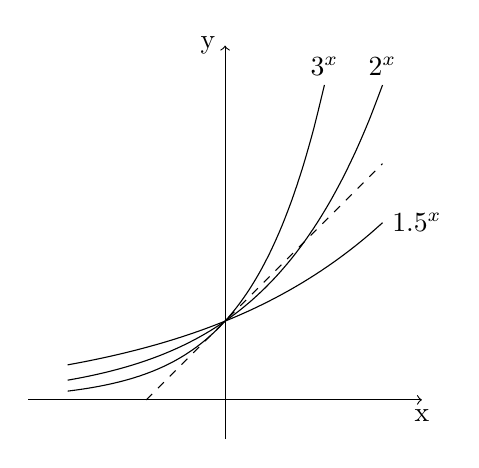
\begin{tikzpicture}
\draw[->] (-2.5, 0) -- (2.5, 0);
\draw (2.5, 0) node[anchor=north]{x};

\draw[->] (0, -0.5) -- (0, 4.5);
\draw (0, 4.5) node[anchor=east]{y};

\draw[domain=-2:2, smooth, variable = \x] plot ({\x}, {pow(1.5, \x)}) node[anchor=west]{\(1.5^x\)};
\draw[domain=-2:2, smooth, variable = \x] plot ({\x}, {pow(2, \x)}) node[anchor=south]{\(2^x\)};
\draw[domain=-2:1.2619, smooth, variable = \x] plot ({\x}, {pow(3, \x)}) node[anchor=south]{\(3^x\)};

\draw[dashed] (-1, 0) -- (2, 3);

\end{tikzpicture}
\caption{Derivace exponenciální funkce}
\end{center}
\label{img:derivace_exponencialni_funkce}
\end{figure}

Na obrázku~\ref{img:derivace_exponencialni_funkce} vidíme několik různých exponenciálních funkcí, všechny procházejí budem \([0, 1]\) protože \(a^0 = 1\). Na obrázku je také čárkovaně zakreslena přímka odpovídající v~tomto bodě tečně funkce s~derivací 1. Vidíme, že existuje základ mocniny, pro kterou bude tato přímka tečnou a~že leží mezi čísly 2 a~3. Tento základ nazveme Eulerovým číslem po slavném matematikovy a~označíme jej \(e\). Pro Eulerovo číslo tedy musí platit:

\begin{equation}
\lim_{dx \to 0} \frac{e^{dx} - 1}{dx} = 1
\end{equation}

Z~něj můžeme Eulerovo číslo vyjádřit:

\begin{equation}
\begin{split}
\lim_{dx \to 0} e^{dx} - 1 = \lim_{dx \to 0} dx \\
\lim_{dx \to 0} e^{dx} = \lim_{dx \to 0} (1 + dx) \\
e = \lim_{dx \to 0} \sqrt[dx]{1 + dx}
\end{split}
\end{equation}

Zavedeme-li substituci \(dx = \frac{1}{n}\), pak dostaneme známý vztah pro výpočet Eulerova čísla:

\begin{equation}
e = \lim_{n \to \infty} \left(1 + \frac{1}{n}\right)^n
\end{equation}

Uvedená limita znamená, že \(n\) roste nade všechny meze, přesnou definici zde nebudeme uvádět. Je zřejmé, že pokud \(n \to \infty\), pak \(dx \to 0\). Například pro \(n = 2^{66}\) dostaneme \(e \approx 2.718281828459045235\).

Proto platí:

\begin{equation}
\frac{\mathrm{d}}{\mathrm{d}x} e^x = e^x
\end{equation}

Inverzní funkcí je přirozený logaritmus \(\ln x\). Proto platí:

\begin{equation}
\ln e^x = x
\end{equation}

\begin{equation}
e^{\ln x} = x; x > 0
\end{equation}

Obecnou exponenciální funkci proto můžeme zapsat

\begin{equation}
a^x = e^{\ln a^x} = e^{x \cdot \ln a}; a > 0
\end{equation}

a~proto

\begin{equation}
\frac{\mathrm{d}}{\mathrm{d}x} a^x = \frac{\mathrm{d}}{\mathrm{d}x} e^{x \cdot \ln a} = e^{x \cdot \ln a} \cdot \ln a = \ln a \cdot a^x
\end{equation}

\subsubsection{Derivace přirozeného logaritmu}

Vyjdeme z~identity

\begin{equation}
e^{\ln x} = x; x > 0
\end{equation}

a~použitím vztahu~\eqref{eq:derivace_inverzni_funkce} získáme

\begin{equation}
\frac{\mathrm{d}}{\mathrm{d}x} \ln x = \frac{1}{e^{\ln x}} = \frac{1}{x}; x > 0
\end{equation}

\subsubsection{Derivace reálné mocniny}

Dříve jsme dokázali vztah \(\frac{\mathrm{d}}{\mathrm{d}x} x^n = n \cdot x^{n-1}\) pro \(x \in \mathbb{R}\) a~\(n \in \mathbb{N}\). Nyní dokážeme, že tento vztah platí i~pro reálné exponenty. Protože platí

\begin{equation}
x^r = e^{\ln x^r} = e^{r \cdot \ln x}; x \in \mathbb{R}^+, r \in \mathbb{R}
\end{equation}

tak proto platí

\begin{equation}
\frac{\mathrm{d}}{\mathrm{d}x} x^r = \frac{\mathrm{d}}{\mathrm{d}x} e^{r \cdot \ln x} = e^{r \cdot \ln x} \cdot r \cdot \frac{1}{x} = x^r \cdot r \cdot \frac{1}{x} = r \cdot x^{r-1}; x > 0
\end{equation}


\subsection{Jak derivovat}

S~využitím tabulky derivací primitivních funkcí a~pravidlem pro derivování složených funkcí lze derivovat čistě mechanicky "zeshora dolů". Zkusme zderivovat například:

\begin{equation}
\frac{\mathrm{d}}{\mathrm{d}x} \left(e^{2x+1} + 3x \right)^3 = ...
\end{equation}

Nejvýše postavenou funkcí je \(a^3\) s~\(a = e^{2x+1} + 3x\). Je to ta funkce, kterou bychom při vyčíslování výrazu vypočítali až nakonec. Víme, že derivace \(x^3\) je \(3 x^2\) a~využijeme pravidlo pro derivování složené funkce:

\begin{equation}
... = 3 \cdot \left(e^{2x+1} + 3x \right)^2 \cdot \frac{\mathrm{d}}{\mathrm{d}x} \left(e^{2x+1} + 3x \right) = ...
\end{equation}

Využijeme pravidlo pro derivaci součtu:

\begin{equation}
... = 3 \cdot \left(e^{2x+1} + 3x \right)^2 \cdot \left(\frac{\mathrm{d}}{\mathrm{d}x} e^{2x+1} + \frac{\mathrm{d}}{\mathrm{d}x} 3x \right) = ...
\end{equation}

První člen je \(e^b\) kde \(b = 2x + 1\), ten opět zderivujeme jako složenou funkci. Na druhý člen využijeme pravidlo pro derivaci součinu funkcí. Jedná se o~speciální případ, kdy jedna funkce je konstantní:

\begin{equation}
... = 3 \cdot \left(e^{2x+1} + 3x \right)^2 \cdot \left(e^{2x+1} \cdot \frac{\mathrm{d}}{\mathrm{d}x} \left(2x+1\right) + 3 \cdot \frac{\mathrm{d}}{\mathrm{d}x} x \right) = ...
\end{equation}

Na první člen použijeme pravidlo pro derivaci součtu. Derivace druhého členu \(x\) je 1:

\begin{equation}
... = 3 \cdot \left(e^{2x+1} + 3x \right)^2 \cdot \left(e^{2x+1} \cdot \left(\frac{\mathrm{d}}{\mathrm{d}x} 2x + \frac{\mathrm{d}}{\mathrm{d}x} 1\right) + 3 \right) = ...
\end{equation}

Derivace členu \(2x\) je 2, už ji nebudu znovu rozepisovat na derivaci součinu. Derivace konstanty 1 je 0. Získáme tak výsledek:

\begin{equation}
... = 3 \cdot \left(e^{2x+1} + 3x \right)^2 \cdot \left(2 e^{2x+1} + 3 \right)
\end{equation}

Tento postup je obecný a~s~trochou cviku lze derivace jednodušších výrazů psát napřímo bez rozepisování mezikroků. 

\subsection{Vícenásobná derivace}

Derivací funkce je funkce, kterou můžeme opět derivovat. Máme-li funkci více proměnných, pak můžeme derivotat podle stejné nebo podle jiné proměnné.

Mějme například funkci \(\mathrm{f}(x) = x^3 y^2\). Pak \(\frac{\partial \mathrm{f}}{\partial x} = 3 x^2 y^2\). Tuto první derivaci můžeme opět derivovat podle \(x\) a~získáme \(\frac{\partial^2 \mathrm{f}}{\partial x^2} = 6 x y^2\). Nebo podle \(y\) a~získáme \(\frac{\partial^2 \mathrm{f}}{\partial xy} = 6 x^2 y\).
Funkci \(f\) můžeme také derivovat podle \(y\) a~získáme \(\frac{\partial \mathrm{f}}{\partial y} = 2 x^3 y\). Derivujeme-li tuto derivaci podle \(x\), tak získáme \(\frac{\partial^2 \mathrm{f}}{\partial yx} = 6 x^2 y\).

Povšimněme si, že \(\frac{\partial^2 \mathrm{f}}{\partial xy} = \frac{\partial^2 \mathrm{f}}{\partial yx}\). To, že nezáleží na pořadí derivování, nyní dokážeme obecně:

\begin{equation}
\begin{split}
\frac{\partial^2 \mathrm{f}}{\partial yx} = \\
\lim_{dx \to 0} \frac{\lim_{dy \to 0} \frac{\mathrm{f}(x+dx, y+dy) - \mathrm{f}(x+dx, y)}{dy} - \lim_{dy \to 0} \frac{\mathrm{f}(x, y+dy) - \mathrm{f}(x, y)}{dy}}{dx} = \\
\lim_{dx \to 0, dy \to 0} \frac{\mathrm{f}(x+dx, y+dy) - \mathrm{f}(x+dx, y) - \mathrm{f}(x, y+dy) + \mathrm{f}(x, y)}{dx \cdot dy} = \\
\lim_{dx \to 0} \frac{\lim_{dy \to 0} \frac{\mathrm{f}(x+dx, y+dy) - \mathrm{f}(x, y+dy)}{dx} - \lim_{dy \to 0} \frac{\mathrm{f}(x+dx, y) - \mathrm{f}(x, y)}{dx}}{dy} = \\
\frac{\partial^2 \mathrm{f}}{\partial xy}
\end{split}
\end{equation}

\subsection{Extrémy funkce}

Lokálním minimem funkce rozumíme bod, ve kterém funkce nabývá lokálně svého minima, tedy všechny funkční hodnoty v~některém nekonečně malém \(\delta\)-okolí jsou větší nebo rovny funkční hodnotě v~tomto bodu. Obdobně definujeme lokální maximum. Lokální extrém je lokální minimum nebo maximum.

\begin{fact}
Mějme funkci \(\mathrm{f}(x)\). Jestliže \(\frac{\partial \mathrm{f}}{\partial x}(x_0) \neq 0\), pak v~bodě \(x_0\) nemůže funkce \(\mathrm{f}\) mít lokální extrém.
Funkce tedy může mít lokální extrém v~bodech, kde je její první derivace rovna 0 nebo kde není definovaná. 
\end{fact}

Intuitivně je věta jasná, pokud má funkce nenulovou první derivaci, pak v~okolí bodu probíhá podle tečny - na jednu stranu roste a~na druhou klesá. Exaktně to dokážeme takto. Vyjdeme z~definice derivace:

\begin{equation}
\frac{\partial \mathrm{f}}{\partial x}(x_0) = \lim_{\mathrm{d}x \to 0} \frac{\mathrm{f}(x + \mathrm{d}x) - \mathrm{f}(x)}{\mathrm{d}x}
\end{equation}

Rozepíšeme-li limitu, tak získáme:

\begin{equation}
\begin{split}
\left| \frac{\mathrm{f}(x_0 + \mathrm{d}x) - \mathrm{f}(x_0)}{\mathrm{d}x} - \frac{\partial \mathrm{f}}{\partial x} \right| < \varepsilon \\
\left| \frac{\mathrm{f}(x_0 + \mathrm{d}x) - \mathrm{f}(x_0) - \frac{\partial \mathrm{f}}{\partial x} \cdot \mathrm{d}x}{\mathrm{d}x} \right| < \varepsilon \\
\left| \mathrm{f}(x_0 + \mathrm{d}x) - \mathrm{f}(x_0) - \frac{\partial \mathrm{f}}{\partial x} \cdot \mathrm{d}x \right| < \varepsilon \cdot | \mathrm{d}x | \\
\end{split}
\end{equation}

Hodnotu \(\varepsilon\) můžeme zvolit libovolnou kladnou, zvolíme tedy \(\varepsilon = \left|\frac{\partial \mathrm{f}}{\partial x} \right|\):

\begin{equation}
\left| \mathrm{f}(x_0 + \mathrm{d}x) - \mathrm{f}(x_0) - \frac{\partial \mathrm{f}}{\partial x} \cdot \mathrm{d}x \right| < \left|\frac{\partial \mathrm{f}}{\partial x}  \cdot \mathrm{d}x \right|
\end{equation}

Uvědomme-si, že levá a~pravá strana nerovnice jsou si rovny, pokud \(\mathrm{f}(x_0 + \mathrm{d}x) - \mathrm{f}(x_0) = 0\).
Uvažujme nejdříve, že součin \(\frac{\partial \mathrm{f}}{\partial x} \cdot \mathrm{d}x\) je kladný. Pak nerovnice bude platit právě tehdy když \(\mathrm{f}(x_0 + \mathrm{d}x) - \mathrm{f}(x_0) > 0\). Uvažujme naopak, že součin \(\frac{\partial \mathrm{f}}{\partial x} \cdot \mathrm{d}x\) je záporný. Pak nerovnice bude platit právě tehdy když \(\mathrm{f}(x + \mathrm{d}x) - \mathrm{f}(x) < 0\). To ale znamená, že pro opačná znaménka \(\mathrm{d}x\) musí být \(\mathrm{f}(x_0 + \mathrm{d}x)\) jednou větší a~podruhé menší než \(\mathrm{f}(x_0)\). Funkce tedy nemůže v~daném bodě mít lokální extrém, protože v~každém (libovolně malém) \(\delta\)-okolí bodu \(x_0\) bude funkce obsahovat hodnoty větší i~menší než \(\mathrm{f}(x_0)\).

Pokud máme funkci více proměnných \(\mathrm{g}(x_1, x_2, ..., x_n)\), pak parciální derivaci vůči kterémukoli z~nich získáme tak, že ostatní parametry považujeme za konstantní. Nechť derivujeme například vůči parametru \(x_1\). Můžeme tedy uvažovat, že máme funkci jedné proměnné \(\mathrm{f}(x) = \mathrm{g}(x, x_2, ..., x_n)\), přičemž \(\frac{\partial \mathrm{f}}{\partial x} = \frac{\partial \mathrm{g}}{\partial x_1}\). To tedy znamená:

\begin{fact}
Mějme funkci \(\mathrm{g}(x_1, x_2, ..., x_n)\). Jestliže \(\frac{\partial \mathrm{g}}{\partial x_i}(x_{10}, x_{20}, ..., x_{n0}) \neq 0\), pak v~bodě \((x_{10}, x_{20}, ..., x_{n0})\) nemůže funkce \(\mathrm{g}\) mít lokální extrém.
Funkce tedy může mít lokální extrém v~bodech, kde jsou všechny první derivace vůči všem jejím parametrům rovny 0 nebo kde není alespoň jedna z~nich definovaná.
\end{fact}
